\documentclass[a2 paper]{article}
%\usepackage[textwidth=8cm,textheight=5cm]{geometry}
\usepackage{paracol}
\usepackage{pdflscape}
\usepackage{kantlipsum}
\usepackage{lipsum}
\usepackage[margin=.5in]{geometry}

\usepackage[utf8]{inputenc}
\usepackage[TS1,T1]{fontenc}
%\usepackage{fourier, heuristica}
\usepackage{array, booktabs}
\usepackage{graphicx}
\usepackage[x11names,table]{xcolor}
\usepackage{caption}
\DeclareCaptionFont{blue}{\color{LightSteelBlue3}}

\usepackage{caption}
\usepackage{hyperref}
\usepackage[czech]{babel}
%\renewcommand{\thetable}{}
%\setarticletemplate{caption}{\raggedright\insertcaption\par}

\newcommand{\foo}{\color{LightSteelBlue3}\makebox[0pt]{\textbullet}\hskip-0.5pt\vrule width 1pt\hspace{\labelsep}}

\title{Rakousko v~poválečné době}
\author{Dalibor Kramář}

\makeatletter
\let\thetitle\@title
\let\theauthor\@author
\makeatother

\begin{document}
\pagestyle{empty}
\begin{landscape}
\begin{center}
	{\fontsize{1cm}{1cm} \selectfont \textbf{\thetitle}}
\end{center}
\begin{minipage}[c]{\linewidth}
\centering
\begin{minipage}[t]{0.2\linewidth}
	\section*{Mezinárodní instituce\\ v~Rakousku}
	Jelikož se Rakousko stalo neutrálním státem za~studené války, tak se Vídeň stala centrem diplomatických jednání. Ovšem to také znamenalo, že americké i sovětské tajné jednotky zde se vyskytovali v hojné míře.
	\subsection*{OPEC}
	Jedná se o~organicaci čtrnácti států vyvážejících ropu založenou 1960. Jejich sídlo je ve~Vídni od roku 1965, ačkoliv Vídeň není členem společnosti.
	\begin{minipage}[t]{\linewidth}
		\captionof*{figure}{Sídlo~OPEC}
		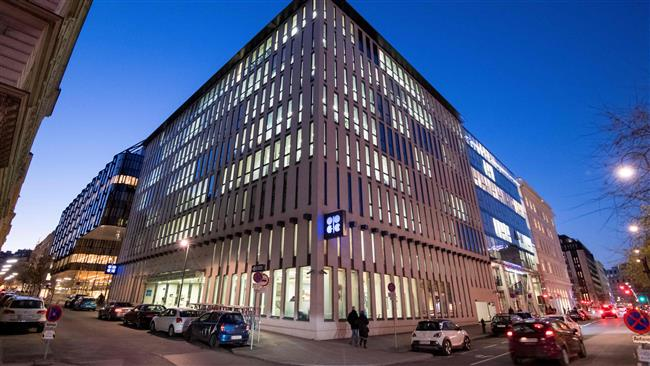
\includegraphics[width=\linewidth]{images/opec.jpg}
	\end{minipage}
	\subsection*{IAEA}
	Mezinárdní agentura pro atomovou energii byla založena 29.~07.~1957 opět se sídlem ve~Vídni. Tato organizace kontroluje zacházení s~jadernou energií, především, je-li využívána mírovou cestou.
	\begin{minipage}[t]{\linewidth}
		\captionof*{figure}{Logo IAEA}
		\centering
		
\includegraphics[width=0.5\linewidth]{images/iaea.png}
	\end{minipage}
	\section*{Další organizace}
	\begin{itemize}
		\item CTBTO (Organizace přípravné komise pro úplný zákaz jaderných testů)
		\item UNIDO (Organizace OSN pro rozvoj průmyslu)
		\item UNODC (Úřad OSN pro drogy a kriminalitu)
		\item OSCE (Organizace pro bezpečnost a spolupráci v Evropě)
	\end{itemize}
\end{minipage}
\hspace{0.5cm}
\begin{minipage}[t]{0.5\linewidth}
	\section*{Rakouko v~letech 1945~--~1955 aneb rakouská cesta ke~svobodě}
	\subsection*{Okupační zóny}
	V důsledku třetí Moskevské smlouvy byly vytvořeny čtyři okupační zóny Rakouska:
	\begin{itemize}
		\item \textbf{americká zóna}: Horní Rakosky (část jižně od dunaje), Salcbursko, malá čast Severního Štýrska
		\item \textbf{britská zóna}: Korutany, Štýrsko, Východní Tyrolsko
		\item \textbf{francouzská zóna}: Vorarlbersko, Severní Tyrolsko
		\item \textbf{sovětská zóna}: Dolní Rakousy, Burgenland, Horní Rakousy (části ležící severně od Dunaje)
	\end{itemize}
	Vídeň byla rovněž rozdělena na~čtyři části, centrum se spravovalo společně. 

	\begin{minipage}[t]{\linewidth}


\captionof*{figure}{Okupační zóny}
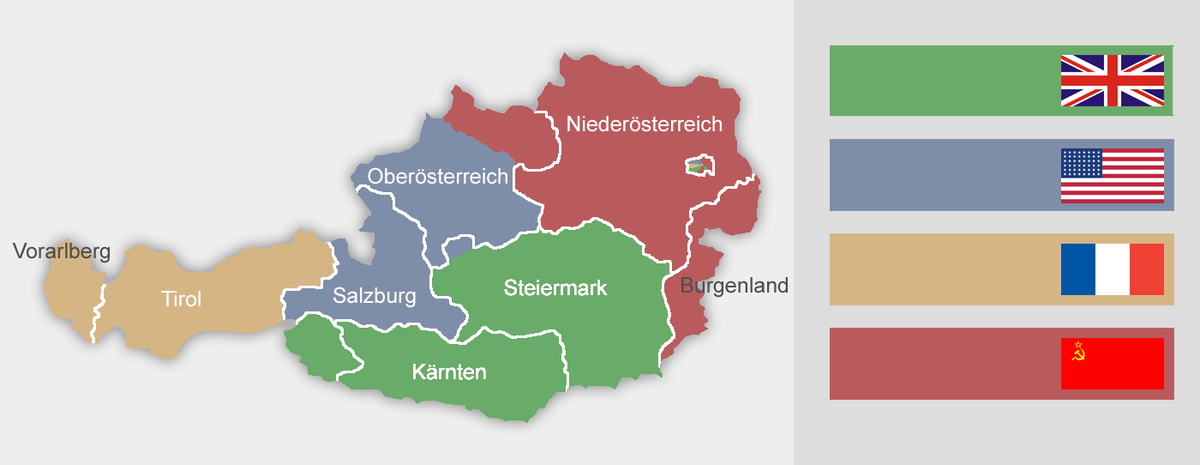
\includegraphics[width=\linewidth]{images/okupacniZony.png}

\end{minipage}
	\subsection*{První svobodné volby}
	25. listopadu 1945 se uskutečnily parlamentní volby. ÖVP (Österreichische Volkspartei, Rakouská lidová strana) získala 49,8\%, SPÖ (Sozialdemokratische Partei Österreichs, Sociálně demokratická strana Rakouska) 44,6\% a KPÖ (Kommunistische Partei Österreichs, komunisté) získali 5,4\%. ÖVP a SPÖ vytvořili koalici a komunisté přišli o podporu ve vládě. Komunisté však stále ovládaly značné množstní odborů.
	\subsection*{Hospodářská situace okolo roku 1950}
	Roku 1947 přijala vláda dohodu o~msdách a cenách, která začala vzbuzovat napětí. Tato situace byla vyřešena o~rok pozdějí přijetím Marshallova plánu. Roku 1950 dochází k~pozastavení Marshallova plánu díky americké válce s~Koreou. Toho využili komunisté a pokusili se vyvolat povstání. 4. října došlo k~rozsáhlým nepokojím ve východním rakousku všetně Vídně. Vláda zareagovala rychle avšak nepoužila pouze vojenskou sílu, ale i odbory. Tím zklidnili napětí a podařilo se jim situaci stabilizovat.
	\subsection*{Rakouské vyjednávání o nezávislosti}
	Od Stalinovy smrti se silně prosazuje myšlenka rakouské suverenity. Avšak sovětští politici v čele s~Molotovem se staví proti a podmiňují neutralitu Rakouska vyřešením situace v~Německu. \par
	Roku 1955 začínalo být zjevné, že západní Německo se připojí k~NATO. Tudíž se dalo předpokládat, že pokud Rakousko nedostane suverenitu, tak se jeho západní čast rovněž stane součástí NATO. Což SSSR nevzhovovalo, neboť plánovali vytvořit \uv{neutrální} úzení (Rakousko, Jugoslávie, \dots). Tato skutečnost měla za následek, že Motolov odvolal  podmíněnost rakouské neutrality vyřešením Německého problému. Požadovali však aby si rakoský stát zachoval neutralitu vůči USA a zakazovali spojení Rakouska s Německem. Nakonec byla 15. května podepsána Rakouská státní smlouva, ve vídeňském zámku Belvedere která zaručovala Rakouskou suverenitu.
	\subsection*{Rakouská politika po roce 1955}
	Aby rakouští demokraté zabránili nástupu KPÖ, rozhodli se pro~tak zvanou velkou koalici ÖVP a SPÖ. To znamená, že tyto starny tvoří společně vládu, i přes to, že jsou navzájem političní oponenti. Tato koalice vládla až do roku 1966, kdy byla přerušena. Pokračuje od roku 1987 do přelomu tisícileti. V roce 1995 došlo k rozštěpení politické scény. Důvoddem byla snížená ochota koalice přešit problémy, což vedlo k postupnému nárůstu opozičních skupin. Následný rozpad vytvořil ekonomickou krizi. (Podobnou jako je česká krize v devadesátých letech).
	\subsection*{Kurt Waldheim}
	Kurt Waldheim byl jeden z~Rakouských politiků, kteří měli nacistickou minulost. Waldheim však tvrdil, že provádědl jen tlumočnka a uředníka a že nevěděl o útocích proti civilnímu obyvatelstvu. V roce 1971 byl jmenovát generálním tajemníkem OSN a byl znám jako kritik Izraele především v průběhu páté Izraelské války. \par
	V roce 1986 byl zvolen prezidentem. Stejný rok se  ukázalo, že lhal o své nacistické minulosti. Byl dokonce usvědčen z páchání válečných zločinů. Většina zemí označila Valdheima jako nežádoucí osobu a byl mu udělen zákaz vstupu do USA. V reakci na~to rakouská vláda sestavila tým historiků, který zkomal Valdheimův život za druhé světové války. Tento výbor potvrdil, že Valdheim věděl pro koho pracuje avšak vyvrátil jeho přímou účast na Válečných zložinech. Tyto události vedly k~tomu, že se rozhodl nekandidovat v dalším volebním období. 
\end{minipage}
\hspace{0.5cm}
\begin{minipage}[t]{0.25\linewidth}
\Large
\renewcommand\arraystretch{1.4}\arrayrulecolor{LightSteelBlue3}
\captionsetup{singlelinecheck=false, font=blue, labelfont=sc, labelsep=quad}
\captionof*{table}{\huge Časová osa}\vskip -1.5ex
%\caption{Timeline}\vskip -1.5ex
\begin{tabular}{@{\,}r <{\hskip 2pt} !{\foo} >{\raggedright\arraybackslash}p{5cm}}
\toprule
\addlinespace[1.5ex]
červenec 1945 & vytvoření okupačních zón\\
listopad 1945 & první svobodné volby\\
\rule{0pt}{9ex}
1948 & přijetí Marshallova plánu\\
\rule{0pt}{6ex}
říjen 1950 & povstání z~důvodu ekonomiky\\
\rule{0pt}{9ex}
březen 1953 & úmrtí Stalina\\
\rule{0pt}{6ex}
květen 1955 & nabytí nezávislosti\\
\rule{0pt}{6ex}
září 1957 & založení IAEA \\
\rule{0pt}{9ex}
září 1960 & založení OPEC\\
\rule{0pt}{15ex}
září 1965 & přesunutí OPEC do~Vídně\\
\end{tabular}
\end{minipage}
\end{minipage}
\vskip 0.5cm
\begin{minipage}[H]{\linewidth}
	\centering
	\subsection*{Kultura}
	\begin{minipage}[t]{0.45 \linewidth}
		\begin{minipage}[t]{0.75\linewidth}
			\subsubsection*{Umění}
			Jedním z nejoblíbenějsím umělců byl zpěvák Johann Hölzel zvaný Falco. Své první album pojmenoval Einzelhaft a mezi nejznámější patři například Falco 3, Emotional nebo Out of the dark. Za svá díla získal mnoho ocenění například Künstler des Jahres~-- ~umělec roku. Dále vyhrál soutěž Bravo Otto v~rocích 1985 a 1986. Zemřel roku 1998 v Dominikánské republice. Posmrtně získal další tři ocenění z ceremonie Amadeus Austrian Music Awards.
		\end{minipage}
	\begin{minipage}[t]{0.2\linewidth}
		\centering
		\captionof*{figure}{Falco}
		\includegraphics[height=3cm]{images/Falco.jpg}
	\end{minipage}
	\end{minipage}
	\begin{minipage}[t]{0.45 \linewidth}
		\begin{minipage}[t]{0.75 \linewidth}
			\subsubsection*{Sport}
			Asi nejpopulárnějším sportovcem v~Rakousku je Niki Lauda. Je to bývalý rakouský pilot Formule 1 a trojnásobný mistr světa z~roků 1975, 1977 a 1984. Potě co ukončil kariéru, se začal věnovat létání, dále komentování závodů a podnikání. \par
			Niki Lauda se objevil ve filmu Rush (Rivalové), který pojednává o~jeho konfliktu s~Jamesem Huntem, dalším závodníkem. V~roce 1976 totiž spolu tito závedníci soupeřili a Niki Lauda měl nehodu. Díky tomu neobájil tento rok titul a rok poté po obhajobě tutulu ukončil kariéru. Avšak v roce 1982 se vrátil a o dva roky později získal třetí titul.
		\end{minipage}
		\begin{minipage}[t]{0.2 \linewidth}
			\centering
			\captionof*{figure}{Falco}
			\includegraphics[height=3cm]{images/niki-lauda.jpg}
		\end{minipage}
	\end{minipage}
\end{minipage}
\end{landscape}
\end{document}